\documentclass[10pt, a4paper]{article}
\usepackage[left=2.00cm, right=2.00cm, top=2.00cm, bottom=2.00cm]{geometry}
\usepackage{supertabular}
\usepackage{graphicx}
\usepackage{float}
\usepackage[fontset=windows]{ctex}
\usepackage{amsmath,amssymb,amsthm}
\usepackage{unicode-math}
\usepackage{verbatim}
\usepackage{multirow}
\usepackage{pifont}
\usepackage{caption}
\usepackage{diagbox}
\usepackage{listings}
\usepackage{algorithm}  
\usepackage{algpseudocode}
\usepackage{booktabs}   
\usepackage{underscore}
\usepackage{xcolor}
\lstset{
  %行号
  numbers=left,
  %背景框
  frame=single,
  rulecolor=\color[rgb]{0.8,0.8,0.8},         % 设置代码框颜色
  breaklines,                                 % 自动将长的代码行换行排版
  extendedchars=false,                        % 解决代码跨页时,章节标题,页眉等汉字不显示的问题
  %背景色
  %backgroundcolor=\color[rgb]{1,1,0.76},
  backgroundcolor=\color[RGB]{245,245,244},
  %样式
  keywordstyle=\bf\color{blue},
  identifierstyle=\bf,
  numberstyle=\color[RGB]{0,192,192},
  commentstyle=\it\color[RGB]{0,96,96},
  stringstyle=\rmfamily\slshape\color[RGB]{128,0,0},
  %显示空格
  showstringspaces=false
}

\setcounter{secnumdepth}{4}
\setcounter{tocdepth}{4}
\newcommand{\whiteding}[1]{\ding{\numexpr171+#1\relax}}
\newcommand\vbf{\symbfit}
\newtheorem{definition}{\hspace{2em}定义}
\newtheorem{theorem}{\hspace{2em}定理}
\renewcommand{\algorithmicrequire}{\textbf{Input:}}  % Use Input in the format of Algorithm  
\renewcommand{\algorithmicensure}{\textbf{Output:}} % Use Output in the format of Algorithm  

\title{\heiti 大作业5\phantom{   }Van der Pauw法测量电阻率}
\author{ 张钰坤 \\  2000011314 \\(C语言实现)}
\date{2022年5月15日}

\begin{document}
    \maketitle
    \tableofcontents
    \newpage

    \section{解题思路}
    本题要求解如下的定解问题:

    \begin{align}
        \text{方程:}&\nabla ^2\phi=0,(x,y)\in \Omega\\
       \text{定解条件:}& \vbf{n}\cdot \nabla\phi=0,(x,y)\in \partial \Omega\\
       & \sigma d\int_C \vbf{n} \cdot \nabla\phi  dl=\pm I,\forall C\subseteq \Omega
   \end{align}

   \subsection{无量纲化}

   选定
   \begin{align*}
       \tilde{\phi}&=\phi/(1V)\\
        \tilde{I}&=\frac{I}{\sigma d(1V)}\\
        \tilde{R}&=\frac{\tilde{U}}{\tilde{I}}
   \end{align*} 

   而所有长度选定某个单位,比如说厘米。

   于是定解问题化为

   \begin{align}
    \text{方程:}&\nabla ^2\tilde\phi=0,(\tilde x,\tilde y)\in \Omega\\
   \text{定解条件:}& \vbf{\tilde n}\cdot \tilde \nabla\tilde \phi=0,(\tilde x,\tilde y)\in \partial \Omega\\
   & \int_C \vbf{\tilde n} \cdot \tilde \nabla\tilde \phi  d\tilde l=\pm \tilde I,\forall C\subseteq \Omega
    \end{align}

    Van der Pauw方程化为

    \begin{align}
        \exp(-\pi\tilde{R}_{AB,DC})+\exp(-\pi\tilde{R}_{AD,BC})=1
    \end{align}

    \subsection{简化条件}
    不失一般性,我们将物理量无量纲化的上标省略:
    \begin{align}
         \text{方程:}&\nabla ^2\phi=0,(x,y)\in \Omega\\
        \text{定解条件:}& \vbf{n}\cdot \nabla\phi=0,(x,y)\in \partial \Omega\\
        & \int_C \vbf{n} \cdot \nabla\phi  dl=\pm I,\forall C\subseteq \Omega
    \end{align}
    
    注意到第三个方程是对无穷个曲线的限制条件,不具有操作性。事实上,第三个方程可以用前两个条件简化。
    
    \begin{figure}[H]
        \centering
        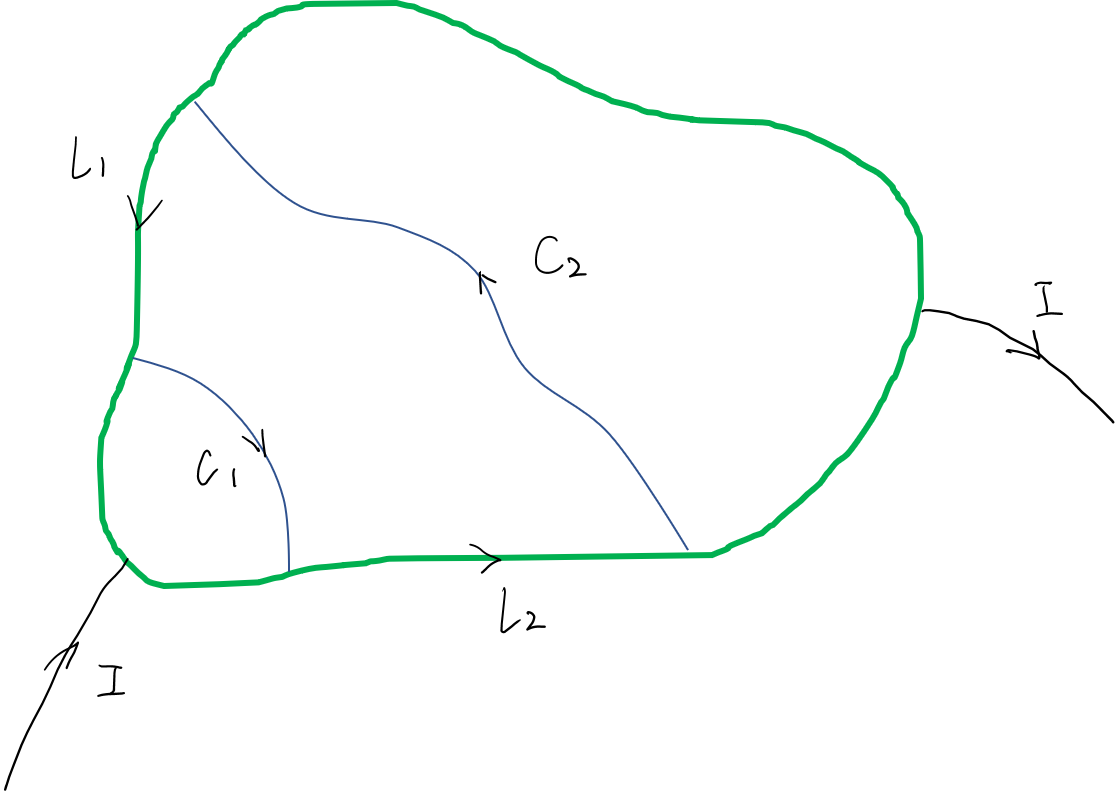
\includegraphics[width=0.4\textwidth]{条件简化示意图1.png}
        \caption{条件简化示意图1}\label{fig:条件简化示意图1}
    \end{figure}

    如示意图1所示,对任意$\Omega$内的曲线$C_1,C_2$,设它们截出的边界为$l_1,l_2$,且$l_1,l_2$不包含源点。那么有

    \begin{align*}
        \oint \vbf{n}\cdot\nabla\phi dl=
        \begin{cases}
            \iint_\Omega \nabla^2\phi dS=0\\
            (\int_{C_1^-}+\int_{C_2^+}+\int_{l_1}+\int_{l_2})\vbf{n}\cdot\nabla\phi dl=(\int_{C_1^-}+\int_{C_2^+})\vbf{n}\cdot\nabla\phi dl
        \end{cases}
    \end{align*}
    其中第一行的等号用到了方程,第二行等号用到了边界条件。

    进而得到

    \begin{align*}
        \int_{C_1}\vbf{n}\cdot\nabla\phi dl=\int_{C_2}\vbf{n}\cdot\nabla\phi dl
    \end{align*}

    根据上面的性质,方程三$\int_C \vbf{n} \cdot \nabla\phi  dl=\pm I,\forall C\subseteq \Omega$可以简化为
    \begin{align*}
        \int_{C_{in}} \vbf{n} \cdot \nabla\phi  dl= I, \int_{C_{out}} \vbf{n} \cdot \nabla\phi  dl= -I
    \end{align*}

    其中$C_{in},C_{out}$是电极附近的一个选定的曲线,如示意图2所示。

    \begin{figure}[H]
        \centering
        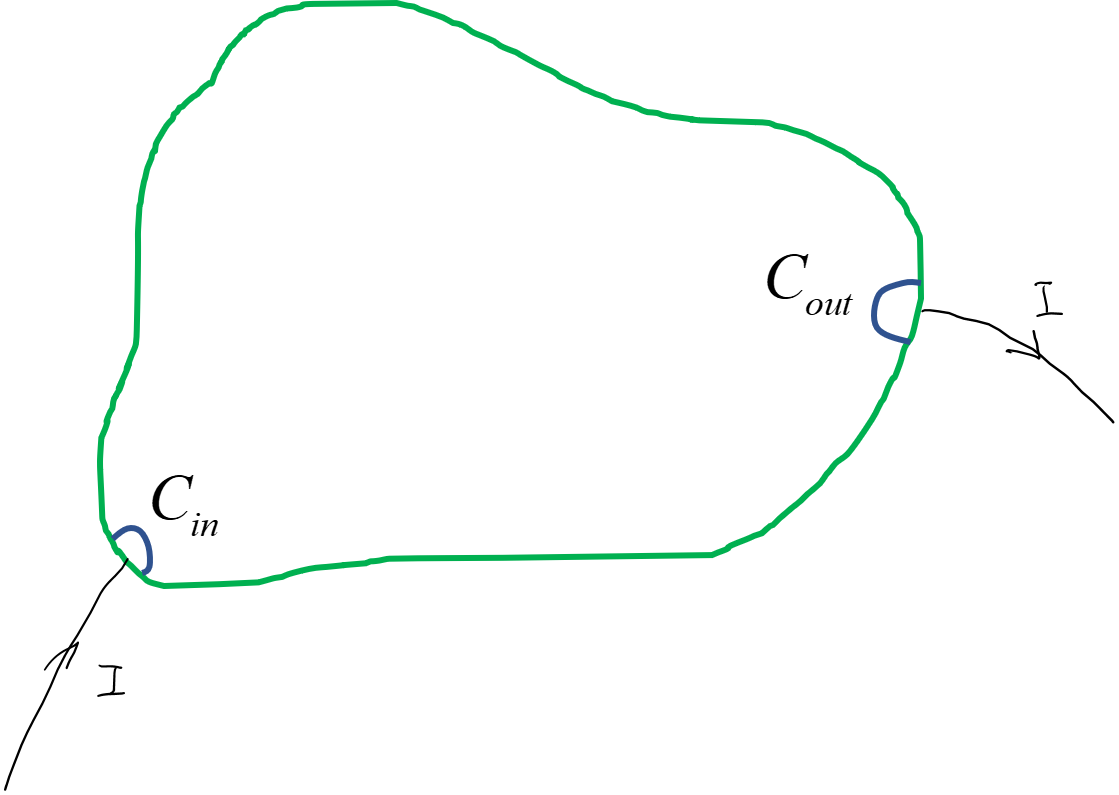
\includegraphics[width=0.4\textwidth]{条件简化示意图2.png}
        \caption{条件简化示意图2}\label{fig:条件简化示意图2}
    \end{figure}

    \subsection{方形网格离散化}
    根据上述讨论,我们确定了数值求解的定解问题:

    \begin{align}
        \text{方程:}&\nabla ^2\phi=0,(x,y)\in \Omega\\
       \text{定解条件:}& \vbf{n}\cdot \nabla\phi=0,(x,y)\in \partial \Omega\\
       & \int_{C_{in}} \vbf{n} \cdot \nabla\phi  dl= I, \int_{C_{out}} \vbf{n} \cdot \nabla\phi  dl= -I
   \end{align}

   本题欲采用有限差分的方法求解,并采用方形网格对求解区域离散化。

   \begin{figure}[H]
    \centering
    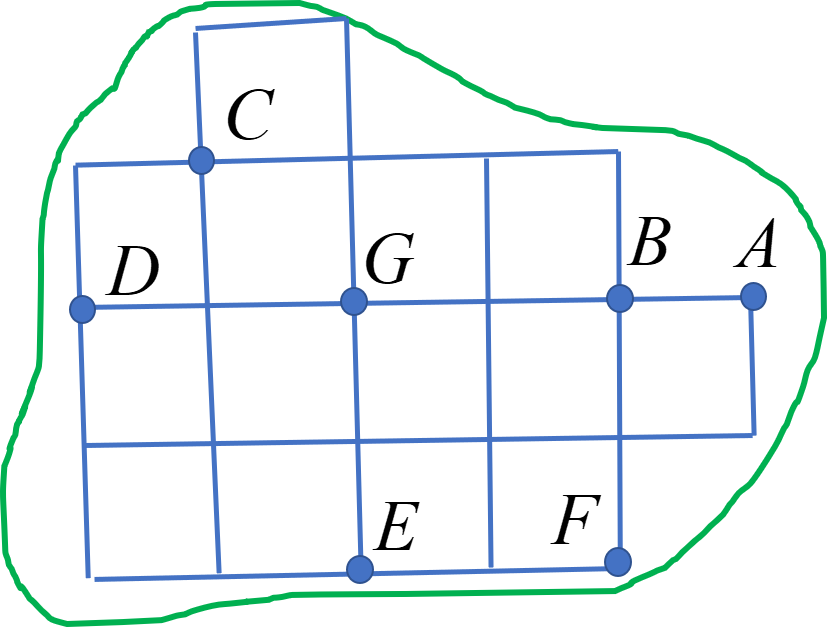
\includegraphics[width=0.4\textwidth]{方形网格离散化区域.png}
    \caption{方形网格离散化区域}\label{fig:方形网格离散化区域}
    \end{figure}

    如上图所示,经过离散化后,我们实际用网格区域代替了原来的区域。我们规定,当网格点上下左右都有格点的时候,认为该格点是内点;当网格上下左右有格点缺失的时候,认为该格点是边界点。例如,上图中ADEF是边界点,BCG是内点。注意这里我们认为BC也是内点。看似当我们用网格区域代替了原来的区域时,BC处在了边界上,但是由于它们常处在凹陷中,离真实物理边界较远,故可以把它们当作内点处理。

    离散化之后给每个格点横纵指标(i,j),将每个格点的电势设为$\phi_{ij}$,进而我们可以分别对内点和边界点满足的方程应用有限差分。

    \subsubsection{内点}

    \begin{figure}[H]
        \centering
        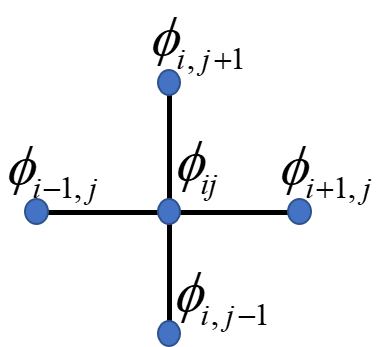
\includegraphics[width=0.2\textwidth]{内点.png}
        \caption{内点}\label{fig:内点}
    \end{figure}

    如图所示,内点满足拉普拉斯方程离散化为
    \[\phi_{i-1,j}+\phi_{i+1,j}+\phi_{i,j-1}+\phi_{i,j+1}-4\phi_{i,j}=0\]

    \subsubsection{边界点}

    \paragraph{无源}

    \textbf{情况1}:格点上下左右只有一个点缺失,如图\ref{fig:方形网格离散化区域}中的DE,此时格点在网格的一条边上。

    \begin{figure}[H]
        \centering
        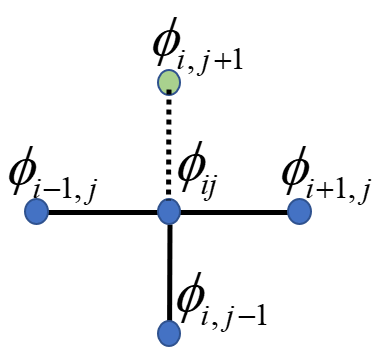
\includegraphics[width=0.2\textwidth]{无源边界点1.png}
        \caption{无源边界点1}\label{fig:无源边界点1}
    \end{figure}

    由于边界点满足$\vbf{n}\cdot \nabla\phi=0$,即电势法向导数为0。我们可以关于直边界$\phi_{i-1,j}\phi_{i,j}\phi_{i+1,j}$把内点$\phi_{i,j-1}$对称出去,得到虚拟点$\phi_{i,j+1}$,如图所示,再由(i,j)点法向导数为0,得到$\phi_{i,j+1}-\phi_{i,j-1}=0$。由于补全了(i,j)点周围的格点,可以由拉普拉斯方程得到
    $\phi_{i-1,j}+\phi_{i+1,j}+\phi_{i,j-1}+\phi_{i,j+1}-4\phi_{i,j}=0$,二者联立,就得到这种边界点的满足的离散化方程:
    \[\phi_{i-1,j}+\phi_{i+1,j}+2\phi_{i,j-1}-4\phi_{i,j}=0\]

    \textbf{情况2}:格点上下左右有2个点缺失,如图\ref{fig:方形网格离散化区域}中的AF,此时格点在网格的某个角上。

    \begin{figure}[H]
        \centering
        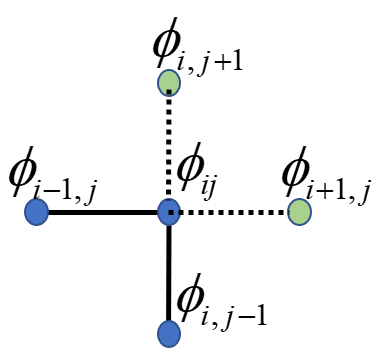
\includegraphics[width=0.2\textwidth]{无源边界点2.png}
        \caption{无源边界点2}\label{fig:无源边界点2}
    \end{figure}

    由于边界点满足$\vbf{n}\cdot \nabla\phi=0$,即电势法向导数为0。我们可以分别关于直边界$\phi_{i-1,j}\phi_{i,j}$和$\phi_{i,j}\phi_{i,j-1}$把内点$\phi_{i-1,j}$和$\phi_{i,j-1}$对称出去,得到虚拟点$\phi_{i+1,j}$和$\phi_{i,j+1}$,如图所示,再由(i,j)点法向导数为0,得到$\phi_{i,j+1}-\phi_{i,j-1}=0$和\phi_{i+1,j}-\phi_{i-1,j}=0。由于补全了(i,j)点周围的格点,可以由拉普拉斯方程得到
    $\phi_{i-1,j}+\phi_{i+1,j}+\phi_{i,j-1}+\phi_{i,j+1}-4\phi_{i,j}=0$,二者联立,就得到这种边界点的满足的离散化方程:

    \[2\phi_{i-1,j}+2\phi_{i,j-1}-4\phi_{i,j}=0\]

    我们不妨在取格点的时候保证,\textbf{边界格点只可能有1或2个上下左右格点缺失,即:边界格点要么在一条边上,要么在一个角上}。进而,所有边界点都可以分成上面两种情况(只差旋转一个角度,分析是类似的)。

    \paragraph{有源}

    根据方程3:$\int_{C_{in}} \vbf{n} \cdot \nabla\phi  dl= I$,可以得出$\vbf{n} \cdot \nabla\phi=\vbf{j}$,即电势的法向导数等于电流密度。

    \textbf{情况1}:格点上下左右只有一个点缺失,此时电流加在网格的一条边上,如下图。

    \begin{figure}[H]
        \centering
        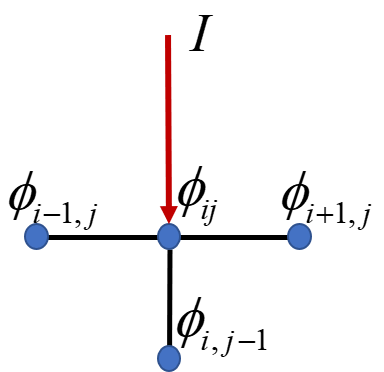
\includegraphics[width=0.2\textwidth]{有源边界点1.png}
        \caption{有源边界点1}\label{fig:有源边界点1}
    \end{figure}

    设格点边长为h,我们不妨设$\phi_{i,j}\phi_{i,j-1}$中点的电流密度为$I/h$,那么有

    \[\frac{\phi_{i,j}-\phi_{i,j-1}}{h}=\frac{I}{h}\]

    于是得到离散化方程

    \[{\phi_{i,j}-\phi_{i,j-1}}={I}\]

    \textbf{情况2}:格点上下左右只有2个点缺失,此时电流加在网格的一个角上,如下图。

    \begin{figure}[H]
        \centering
        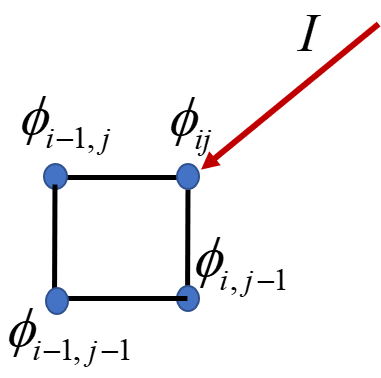
\includegraphics[width=0.2\textwidth]{有源边界点2.png}
        \caption{有源边界点2}\label{fig:有源边界点2}
    \end{figure}

    设格点边长为h,我们不妨设$\phi_{i,j}\phi_{i-1,j-1}$中点的电流密度为$I/h$,那么有

    \[\frac{\phi_{i,j}-\phi_{i-1,j-1}}{\sqrt{2}h}=\frac{I}{\sqrt{2}h}\]

    于是得到离散化方程

    \[{\phi_{i,j}-\phi_{i-1,j-1}}={I}\]

    \subsection{SOR法/Gauss-Seidel法求解线性方程组}

    根据前一节的分析,我们用方形网格离散化待求解区域,设出每个格点上的电势$\phi_{ij}$。经过讨论,这些格点分为三大类:内点,无源边界点,有源边界点。每种情况都可以给出以这些格点为中心的线性方程。因此,有多少个格点,就有多少个未知数,多少个线性方程,进而可以通过解线性方程组的方式,求出所有格点的电势值。

    将$\phi_{ij}$按一定顺序排列成一个向量$\vbf{x}$,线性方程组可以写为

    \[\vbf{Ax}=\vbf{b}\]

    注意到A是一个大型极端稀疏矩阵。因为,想要求解的电势十分精确的反应真实物理情景,有限差分只有在格子取得很小的情况下才能作为导数的近似,这会使得未知数$\phi_{ij}$数量庞大。但是根据前节的讨论,每个格点对应的方程,之和自身和周围的4项相关,说明矩阵A中每行只有至多5个元素非0。故,A大型且稀疏。

    于是我们采用SOR法/Gauss-Seidel法求解。这会遇到两个问题:
    
    \textbf{问题1}:SOR法/Gauss-Seidel法需要矩阵对角元全部非0。

    \textbf{问题2}:由于A规模巨大,难以储存;并且即便储存了,在迭代过程中也会遇到0和数的乘法这种不必要的运算。(下面的估算说明存储A的不值当:假设有一万个格点,那么矩阵A是10000*10000的,如果用二维double数组存储,共占据$8\times10^8B=800MB$内存!并且这个矩阵元素中大部分都是0,有多大部分呢?每行10000个元素最多有5个不是0,那么有9995/10000=$99.95\%$空间浪费掉了!)

    \subsubsection{解决 \textbf{问题1}的办法}

    解决 \textbf{问题1}的办法是:选定$\phi_{ij}$在$\vbf{x}$中的排列次序,那么让$\phi_{ij}$在$\vbf{x}$中由上到下的排列次序,与(i,j)满足的线性方程在$\vbf{A}$中由上到下的排列次序相同。由于(i,j)满足的线性方程一定含有$\phi_{ij}$项,那么对角元一定非零。

    比如说,$\phi_{1,2}$在$\vbf{x}$中是第5个,那么A的第5行就去记录以(1,2)点为中心的方程系数,以(1,2)是内点为例,去记录方程$\phi_{0,2}+\phi_{2,2}+\phi_{1,1}+\phi_{1,3}-4\phi_{1,2}=0$的系数。

    \subsubsection{解决 \textbf{问题2}的办法}

    解决 \textbf{问题2}的办法是:不储存矩阵,而把每一步迭代写成函数,这样既不用储存矩阵,又不用计算许多0和数的乘法。

    参考SOR算法\cite{ref1},

    计
    \[A=\begin{pmatrix}
        \vbf{\alpha_1}\\
        \vbf{\alpha_2}\\
        \vdots\\
        \vbf{\alpha_n}
    \end{pmatrix}\]

    SOR算法的每次迭代可以写为

    \begin{align*}
        \begin{cases}
            {x}_i^{(k+1)}=x_i^{(k)}+\Delta x_i,\\
            \Delta x_i=\omega(b_i-\vbf{\alpha}_i^\top \vbf{x})/A(i;i),\\
            i=1,2,\cdots,n;k=1,2,\cdots;\omega\text{为松弛因子}
        \end{cases}
    \end{align*}

    为简便起见可以让A对角元都为-4,然后可以写一个函数计算$\vbf{\alpha}_i^\top \vbf{x}$。

    \begin{algorithm}[H]  
        \caption{AmX函数,计算$\vbf{\alpha}_i^\top \vbf{x}$}  
        \label{alg:AmX函数}  
        \begin{algorithmic}[1]  
        \Require  
            行数 m,待求解向量 x; 
        \Ensure  
            内积$\vbf{\alpha}_m^\top \vbf{x}$;
        \State 通过m的值确定这一行系数对应的方程中心点(i,j)。(因为要选定一定顺序排列$\phi_{i,j}$,而且系数矩阵A每行的排列与这个顺序相同,见“解决问题1的办法”);

        \If{(i,j)是有源边界点(通电流的点)}
            \State 按照有源边界点方程,用这些系数*对应x中的分量再相加,返回这个值。
        \Else
            \State (i,j)是无源边界点或内点;
            \State 由于无源边界点和内点上的方程本质都是拉普拉斯方程(见“方形网格离散化”),因而二者可以统一,并通过一些判断条件,把想要求的值算出来,下面实现这一点。

            \State 设一个变量s临时储存待求内积;s=0;
            
            \State 因为(i,j)项对应的系数一定是-4,所以s+=$-4\phi_{i,j}$

            \If{(i+1,j)在界外}
                \State (i-1,j)一定在界内,并且由于对称性,(i-1,j)的系数一定是2,故s+=$2\phi_{i-1,j}$
            \EndIf

            \If{(i-1,j)在界外}
                \State (i+1,j)一定在界内,并且由于对称性,(i+1,j)的系数一定是2,故s+=$2\phi_{i+1,j}$
            \EndIf
            
            \If{(i,j+1)在界外}
                \State (i,j-1)一定在界内,并且由于对称性,(i,j-1)的系数一定是2,故s+=$2\phi_{i,j-1}$
            \EndIf

            \If{(i,j-1)在界外}
                \State (i,j+1)一定在界内,并且由于对称性,(i,j+1)的系数一定是2,故s+=$2\phi_{i,j+1}$
            \EndIf

            \If{(i+1,j)不在界外且$\phi_{i+1,j}$没有在之前计入过s}
                \State (i-1,j)的系数一定是1,故s+=$\phi_{i-1,j}$
            \EndIf

            \If{(i-1,j)不在界外且$\phi_{i-1,j}$没有在之前计入过s}
                \State (i+1,j)的系数一定是1,故s+=$\phi_{i+1,j}$
            \EndIf
            
            \If{(i,j+1)不在界外且$\phi_{i,j+1}$没有在之前计入过s}
                \State (i,j-1)的系数一定是1,故s+=$\phi_{i,j-1}$
            \EndIf

            \If{(i,j-1)不在界外且$\phi_{i,j-1}$没有在之前计入过s}
                \State (i,j+1)的系数一定是1,故s+=$\phi_{i,j+1}$
            \EndIf

            \State\Return s
        \EndIf
        \end{algorithmic}  
      \end{algorithm}

    值得注意的是,对于不同形状的导体,不同的电极接入位置,电极方程都略有不同,但好处是内点和无源边界点的处理是兼容的,可以参考源代码中(double) AmX(int, vector* )函数。

    \subsection{遍历格点并寄存位置}

    在上节算法的实现中,我们认为$\phi_{i,j}$通过一定顺序排列好了,并且我们需要经常通过$\phi_{i,j}$的排列序号得到位置坐标(i,j),和通过位置坐标(i,j)确定排列序号。这说明我们需要记录这种映射关系。另外,对于不同形状的导体,如何构造格点是一个问题。我们将在本节中解决这两个问题。
    
    \subsubsection{第一问方形导体}

    方形导体的格子可以直接划分,举个简单的例子,取格子边长0.5,划分3*2的长方形,那么将划出(7*5=35)个格子,选定如下的排列方式。

    \[\begin{matrix}
    28    & 29    & 30    & 31    & 32    & 33    & 34 \\
    21    & 22    & 23    & 24    & 25    & 26    & 27 \\
    14    & 15    & 16    & 17    & 18    & 19    & 20 \\
    7     & 8     & 9     & 10    & 11    & 12    & 13 \\
    0     & 1     & 2     & 3     & 4     & 5     & 6 
    \end{matrix}\]

    那么容易定出格点位置和序号的函数关系。

    一般的,取格子边长h,划分3*2的长方形,可以计算出NX=3/h,NY=2/h。于是划分出(NX+1)*(NY+1)个格子,选定和例子一样的排列方式。

    \[\begin{matrix}
    NY*(NX+1)&\cdots&NY*(NX+1)+NX\\
    \vdots& & \vdots\\
    0& \cdots& NX
    \end{matrix}\]

    可以计算出位置(i,j)(i=0,1,...,NX;j=0,1,...,NY)与序号l(l=0,1,...,(NX+1)*NY+NX)的函数关系:

    \begin{align*}
        l&=i+j(NX+1)\\
        i&=l\%(NX+1)\\
        j&=[l/(NX+1)]
    \end{align*}

    \subsubsection{具有中心对称和轴对称的曲线边界}

    第二、三、四问中的导体形状都是具有中心对称和轴对称性质的,我们不妨把曲线的对称中心放在原点,只在第一象限内划分格子,进而可以对称到其余象限中。

    \begin{figure}[H]
        \centering
        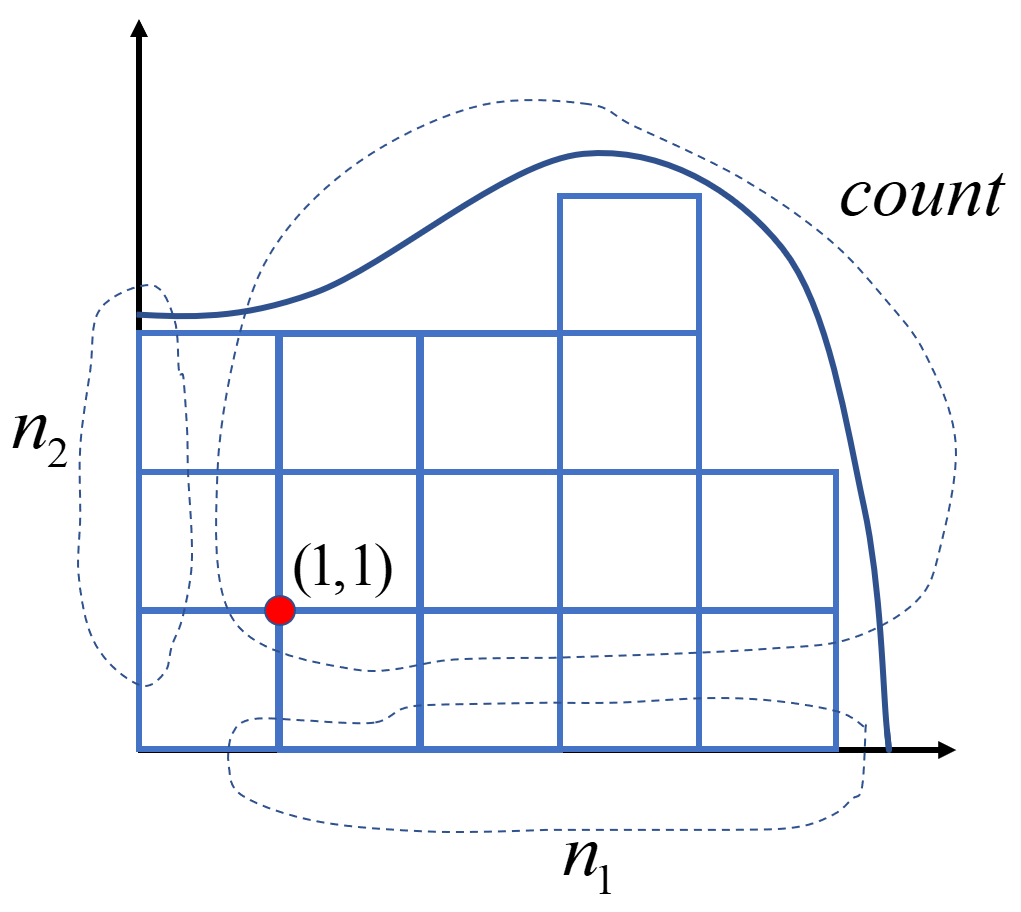
\includegraphics[width=0.6\textwidth]{构造格点示意图.png}
        \caption{构造格点示意图}\label{fig:构造格点示意图}
    \end{figure}

    如上图所示,我们只需要数出上图中三个虚线框中各有多少个格点(count个,n1个,n2个),就可以得到总格点数4*count+2*(n1+n2)+1。

    怎样去数格点呢?我们通过逐行搜索的方式遍历第一象限内所有格点。起点设在(1,1),每次向右踏一步,直到走到了曲线外,我们就回到i=1但是纵指标增加了1,在往上一行继续搜索,直到一整行都没有点在曲线内为止。

    在这个搜索过程中我们可以得到许多离散后的网格信息,不仅限于图中的count,n1,n2,我们还可以得到横向最大格数,纵向最大格数,曲线与y=x交点的近似格点位置(第四问),曲边中点近似格点位置(第二问)等等,详情见每一问的源代码。

    我们通过遍历确定了格点,接下来就可以按照一定顺序给格点编号,并用数组记录三个数(序号l,横指标i,纵指标j)的关系。

    这三个数组分别是:
    
    ltoi[],一维数组,记录每个l对应的i;
    
    ltoj[],一维数组,记录每个l对应的j;
    
    ijtol[][],二维数组,记录(i,j)位置的序号l,相当于是把整个格点图画了下来,由于边界不规则而二维数组是标准的矩形,所以一些数组元素表示导体外的点,可以置为-1,另外由于i,j可能取负数,但数组元素的序号非负,因此可以做适当的平移加以储存,这里不过多赘述,详情见源代码。

    我们采用如下顺序编号:

    1、原点;

    2、x轴:每一次先后标记正负半轴对称位置的两个值,绝对值从小到大;

    3、y轴:每一次先后标记正负半轴对称位置的两个值,绝对值从小到大;

    4、象限内的点:按照数格点时的遍历方式,在第一象限遍历,每遍历到一个点,根据对称性依次把四个象限对称位置的点全部标记。

    这样我们就完成了三个数组的初始化,进而我们可以随时取用l与(i,j)的对应信息。

    我们可以把ijtol[][]打印出来,欣赏一下格点化的成果。

    这里为了演示方便,步长取得比较大。

    第二问,步长0.1

    \begin{figure}[H]
        \centering
        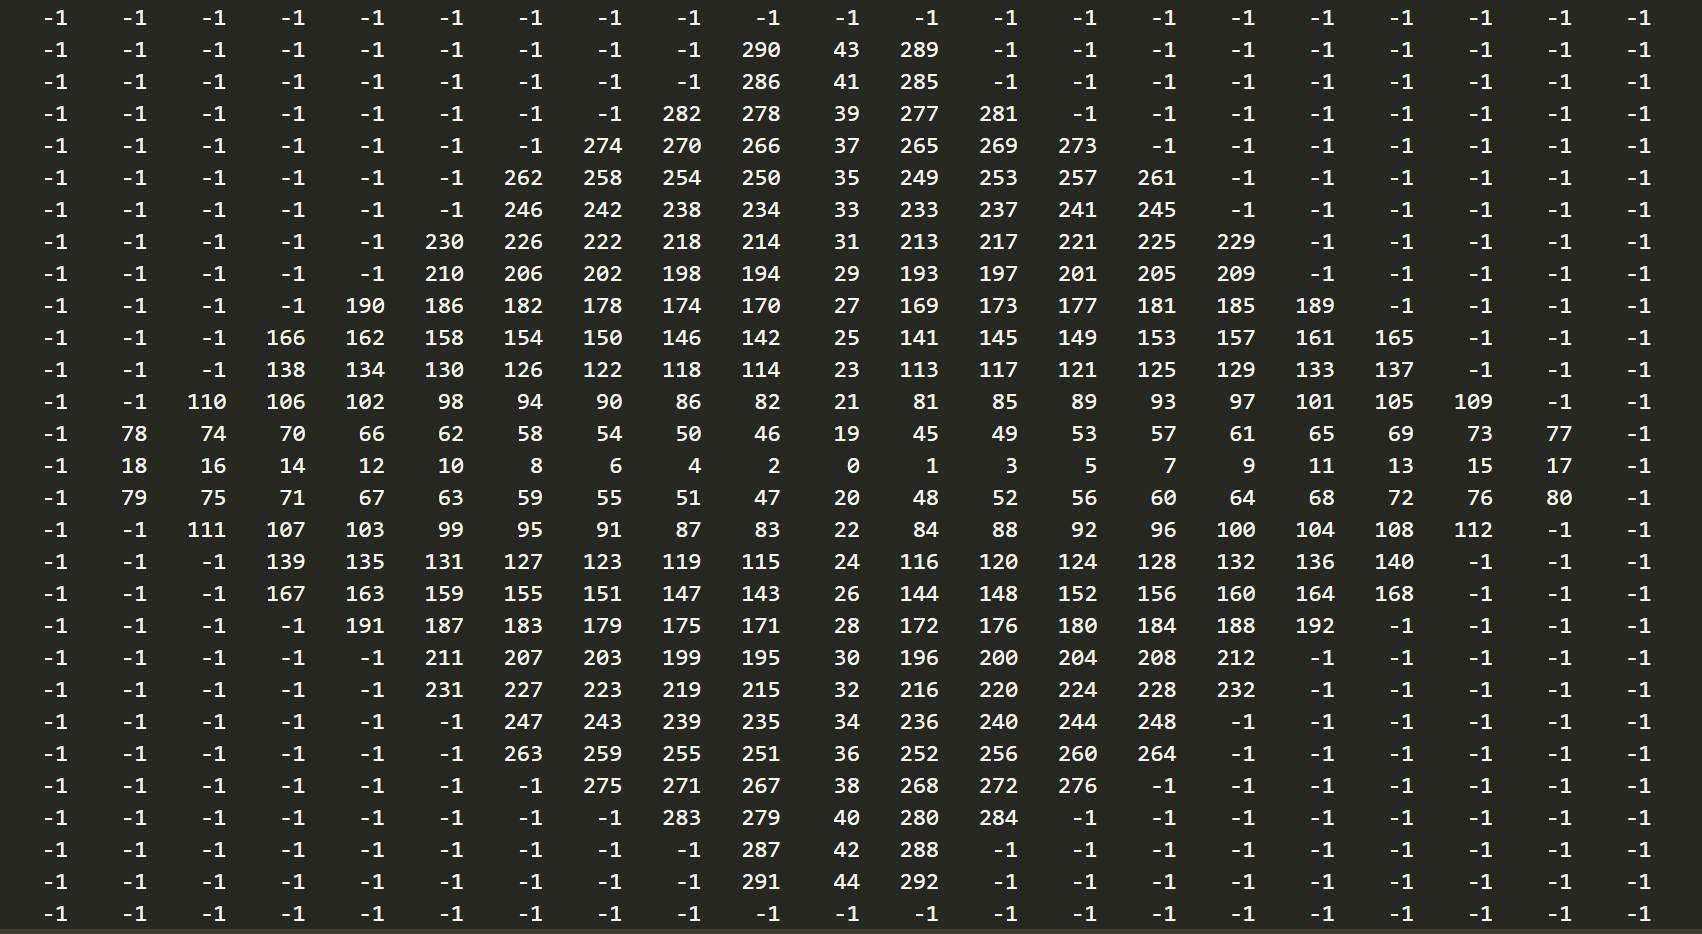
\includegraphics[width=1.0\textwidth]{第二问格点划分示意.png}
        \caption{第二问格点划分示意}\label{fig:第二问格点划分示意}
    \end{figure}

    第三问,步长0.1

    \begin{figure}[H]
        \centering
        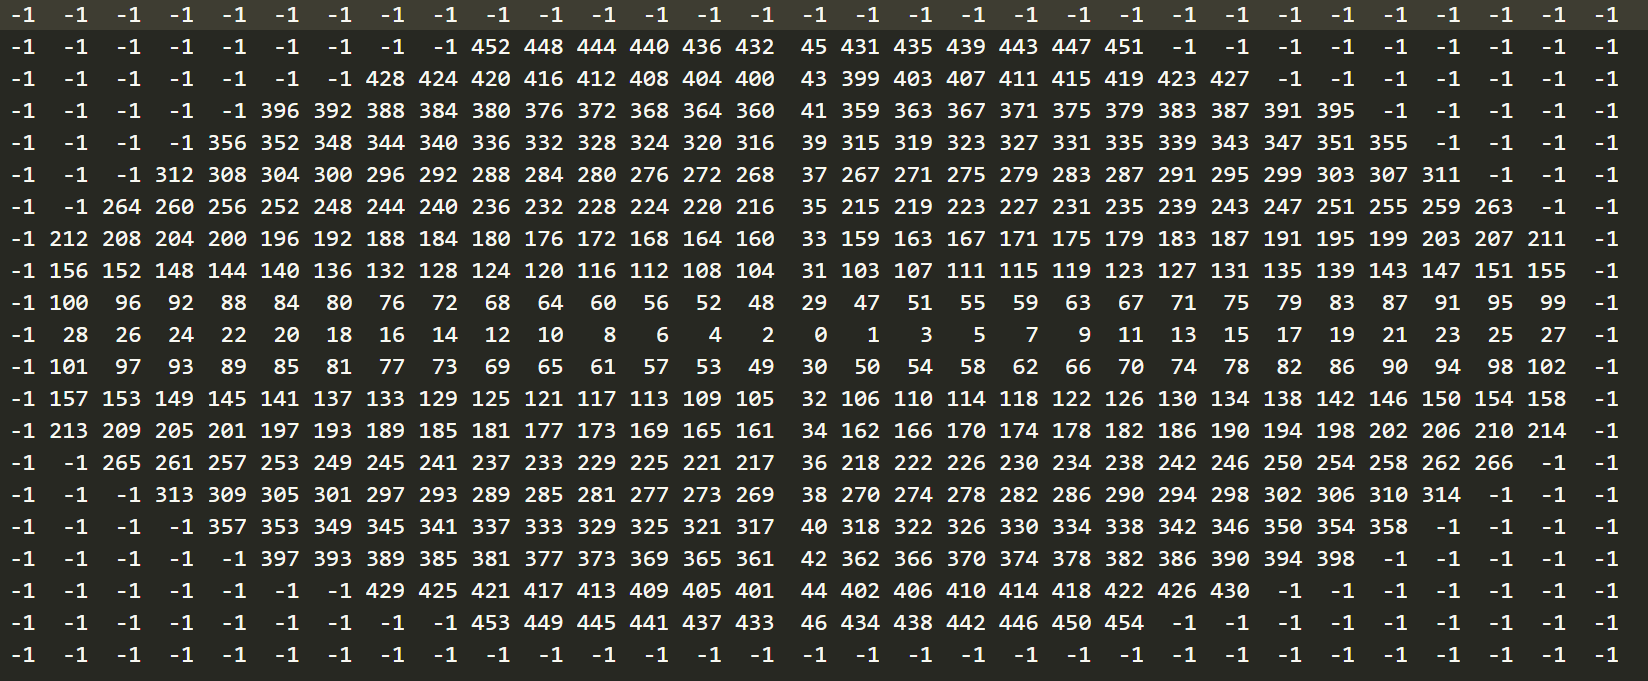
\includegraphics[width=1.0\textwidth]{第三问格点划分示意.png}
        \caption{第三问格点划分示意}\label{fig:第三问格点划分示意}
    \end{figure}

    第四问,步长0.3

    \begin{figure}[H]
        \centering
        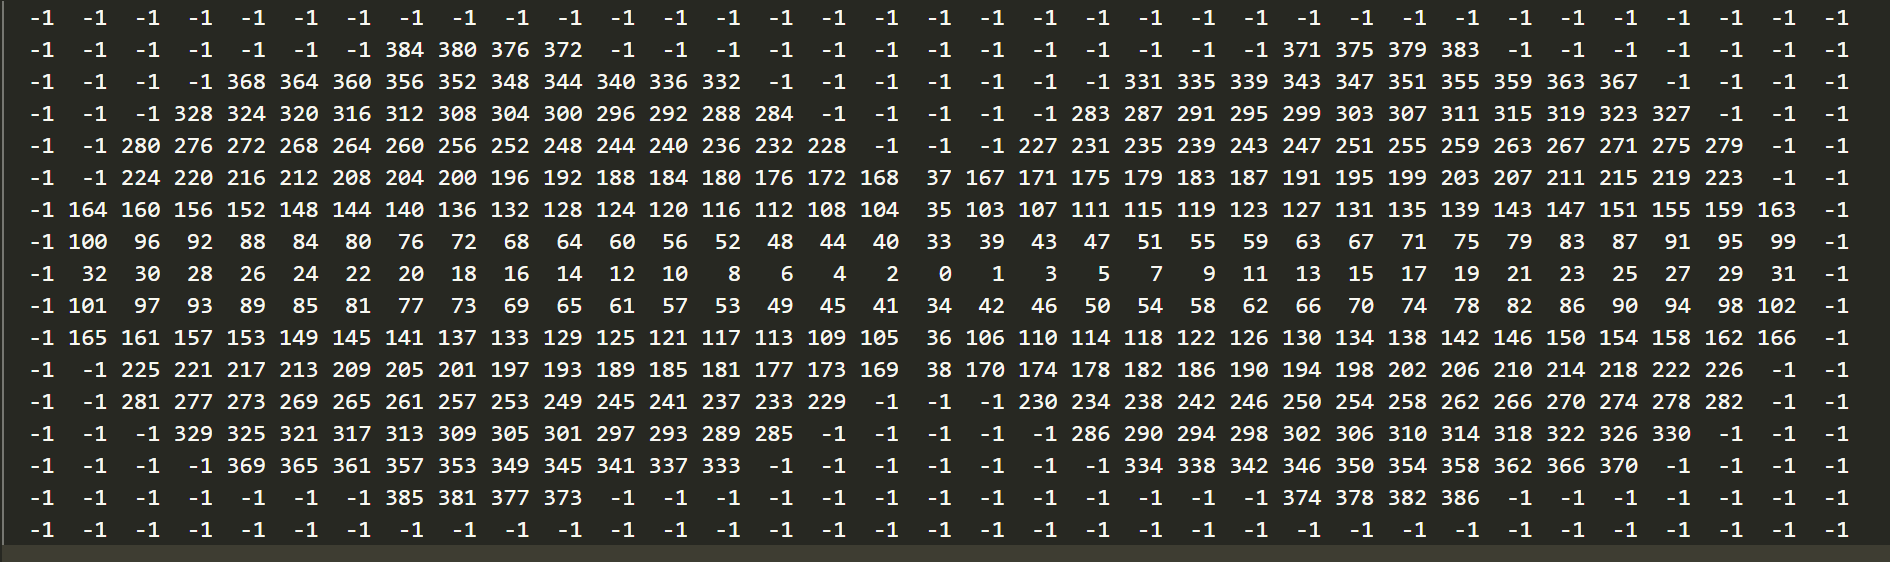
\includegraphics[width=1.0\textwidth]{第四问格点划分示意.png}
        \caption{第四问格点划分示意}\label{fig:第四问格点划分示意}
    \end{figure}

    \section{源代码}

    \textbf{为方便计算取I=1}


    所有C源文件在code文件夹,输出txt文本(打印出绘制等高线图的原始数据,即打印出ijtol[][]矩阵,其中为方便mathematica作图,-1用复数-1+I代替)在data文件夹。
    对应关系如下:

    \begin{table}[H]
        \centering
        \begin{tabular}{|c|c|c|c|}
            \hline
                        & code            & data                      & 对应下节中的图 \\ \hline
            \multirow{2}{*}{第一问} & "q1.c"          & "q1\_NX=300.txt"          & Q1(1)   \\ \cline{2-4} 
                        & "q1\_inverse.c" & "q1\_NX=300\_inverse.txt" & Q1(2)   \\ \hline
            \multirow{2}{*}{第二问} & "q2.c"          & "q2\_H=0.01.txt"          & Q2(1)   \\ \cline{2-4} 
                        & "q2\_inverse.c" & "q2\_H=0.01\_inverse.txt" & Q2(2)   \\ \hline
            \multirow{2}{*}{第三问} & "q3.c"          & "q3\_H=0.01.txt"          & Q3(1)   \\ \cline{2-4} 
                        & "q3\_inverse.c" & "q3\_H=0.01\_inverse.txt" & Q3(2)   \\ \hline
            \multirow{2}{*}{第四问} & "q4.c"          & "q4.txt"                  & Q4(1)   \\ \cline{2-4} 
                        & "q4\_inverse.c" & "q4\_inverse.txt"         & Q4(2)   \\ \hline
        \end{tabular}
        \end{table}

    \textbf{注意:在C编译环境可以运行上述代码,只是每个代码中读写的txt文件需要重新更改路径!!}

    另外,有关松弛因子的选取,这里只是数值估算出的。

    具体方式是,选取一个大一点的步长做测试,这时矩阵维数较小,可以快速出结果。由于改变步长只是对矩阵进行了放缩,可以认为矩阵的性质大致不变,因而可以对小矩阵测试不同的松弛因子,输出迭代次数,然后选取次数最小的松弛因子作为正式的松弛因子。代码中所示松弛因子的就是这种数值计算的近似估计,效果是显著的,运行时间可以缩短几倍。

    \section{结果展示}

    数据代码和对应的图关系见上节对应表格,这里用来绘制图片的mathematica文件"plot.nb"也在附件中。

    \subsection{第一问}
    \begin{figure}[H]
        \centering
        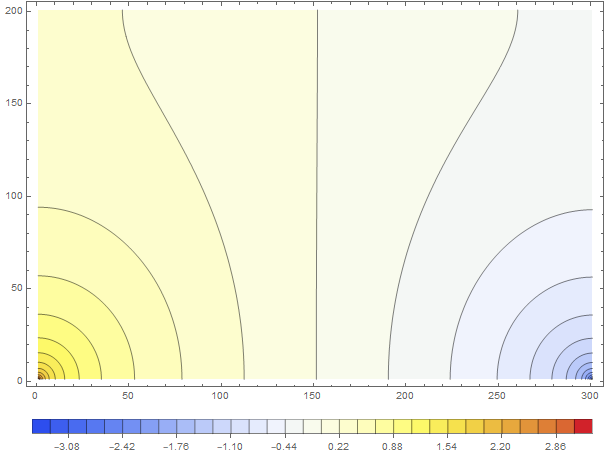
\includegraphics[width=0.4\textwidth]{Q1(1).png}
        \caption{Q1(1)}\label{fig:Q1(1)}
    \end{figure}
    \begin{figure}[H]
        \centering
        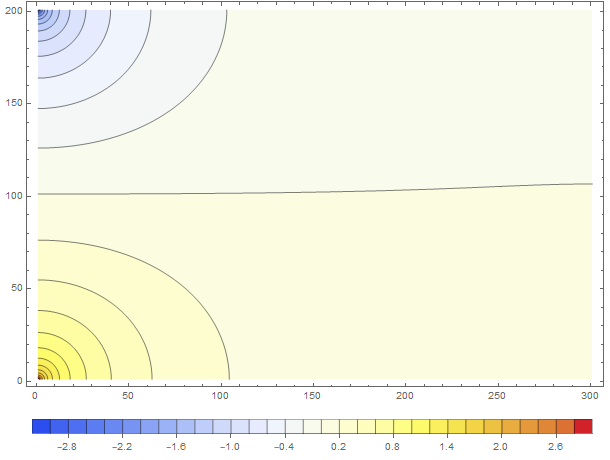
\includegraphics[width=0.4\textwidth]{Q1(2).png}
        \caption{Q1(2)}\label{fig:Q1(2)}
    \end{figure}

    \begin{align*}
        R_1&=(0.248355-(-0.242514))/1\\
        R_2&=(0.017833 - (-0.014927))/1\\
        &E^{-\pi R_1}+E^{-\pi R_2}=1.11613
    \end{align*}

    \subsection{第二问}
    \begin{figure}[H]
        \centering
        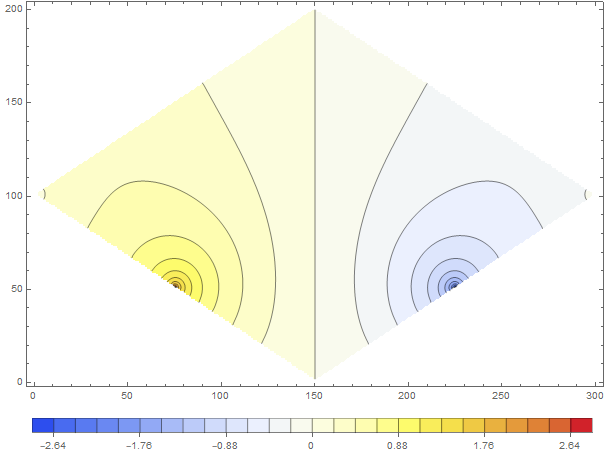
\includegraphics[width=0.4\textwidth]{Q2(1).png}
        \caption{Q2(1)}\label{fig:Q2(1)}
    \end{figure}
    \begin{figure}[H]
        \centering
        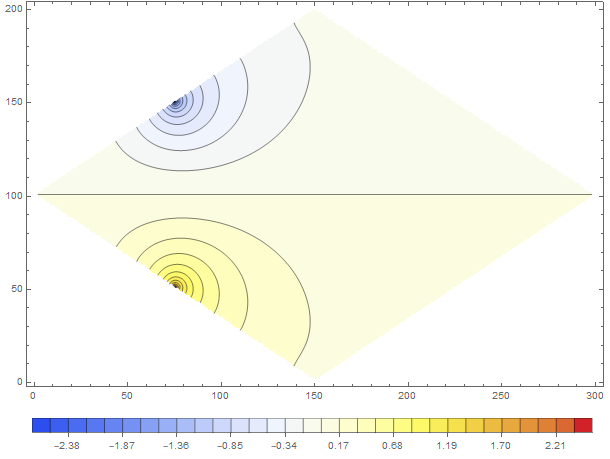
\includegraphics[width=0.4\textwidth]{Q2(2).png}
        \caption{Q2(2)}\label{fig:Q2(2)}
    \end{figure}

    \begin{align*}
        R_1&=(0.293313 -(-0.293313))/1\\
        R_2&=(-(-0.033495) + 0.033495)/1\\
        &E^{-\pi R_1}+E^{-\pi R_2}=0.968566
    \end{align*}

    \subsection{第三问}
    \begin{figure}[H]
        \centering
        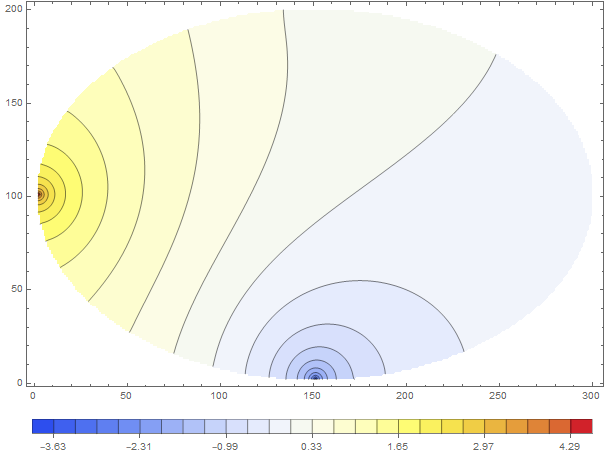
\includegraphics[width=0.4\textwidth]{Q3(1).png}
        \caption{Q3(1)}\label{fig:Q3(1)}
    \end{figure}
    \begin{figure}[H]
        \centering
        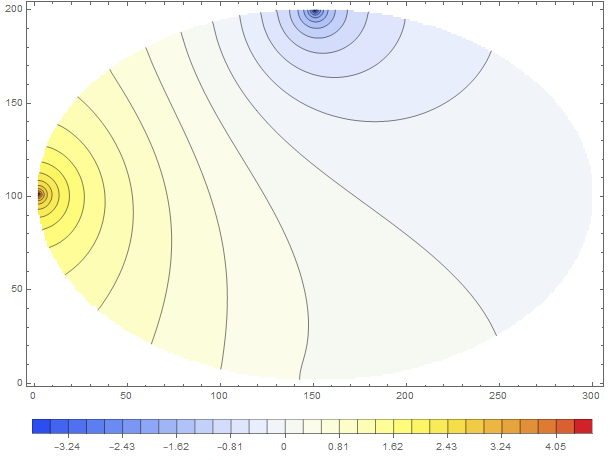
\includegraphics[width=0.4\textwidth]{Q3(2).png}
        \caption{Q3(2)}\label{fig:Q3(2)}
    \end{figure}

    \begin{align*}
        R_1&=(0.129034 - (-0.048891))/1\\
        R_2&=(0.129034 - (-0.048891))/1\\
        &E^{-\pi R_1}+E^{-\pi R_2}=1.1436
    \end{align*}

    \subsection{第四问}
    \begin{figure}[H]
        \centering
        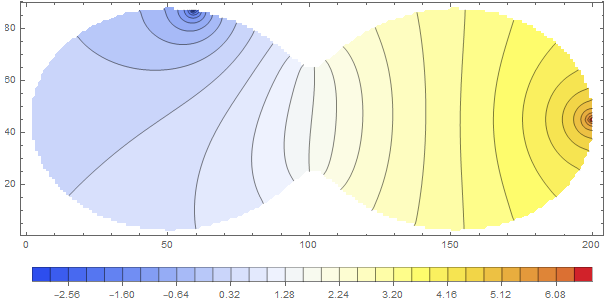
\includegraphics[width=0.6\textwidth]{Q4(1).png}
        \caption{Q4(1)}\label{fig:Q4(1)}
    \end{figure}
    \begin{figure}[H]
        \centering
        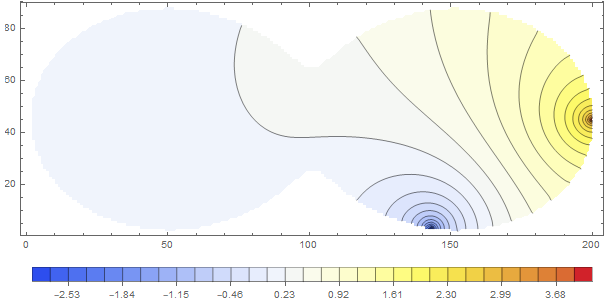
\includegraphics[width=0.6\textwidth]{Q4(2).png}
        \caption{Q4(2)}\label{fig:Q4(2)}
    \end{figure}

    \begin{align*}
        R_1&=(2.985171-1.656232 )/1\\
        R_2&=(0.215642-0.197188 )/1\\
        &E^{-\pi R_1}+E^{-\pi R_2}=0.959049
    \end{align*}

    \begin{thebibliography}{99}  
        \bibitem{ref1}李庆扬,王能超,易大义:数值分析,194页,2008年12月第五版
    \end{thebibliography}

\end{document}